\documentclass[11pt,a4paper,oneside]{article}
\usepackage{graphicx}
\usepackage[usenames,dvipsnames]{xcolor}
\usepackage[section]{placeins}
\usepackage{fancyhdr}
\usepackage{hyperref}
\hypersetup{
    colorlinks,
    citecolor=RoyalBlue,
    filecolor=RoyalBlue,
    linkcolor=RoyalBlue,
    urlcolor=RoyalBlue
}
\usepackage[all]{hypcap}
\pagestyle{fancyplain}

\begin{document}
\lhead{Infographics Generator}
\rhead{Project Plan}
\begin{titlepage}



\begin{center}


\includegraphics[width=1\textwidth]{images/sponsor-logo.png}\\[1cm]    

{ \huge \bfseries Infographics Generator}\\[0.4cm]
{ \large \bfseries Project Plan}\\[0.4cm]

Louis Bodnar\\
Peter Chen\\
Lok Cheung\\
Kevin Shreve\\


\vfill

{\large \today}

\end{center}

\end{titlepage}

\tableofcontents

\newpage

%\listoffigures

%\newpage

\section{Executive Summary}


Over three decades ago, a professor at Wayne State University took on a challenge that Cadillac deemed unsolvable. That professor was Jim Anderson. His computer-generated dot maps gave Cadillac's marketing department a competitive advantage by allowing them to easily visualize dealership locations across the nation. Jim began using the power of computers to analyze these networks of dealerships and started a company that specialized in the planning and management of these networks. Thus, Urban Science was born.\\


Urban Science is now an international company, headquartered in Detroit, Michigan. They assist nearly every original equipment manufacturer (OEM) in over 60 countries. Our job is to design a web application to show OEMs monthly performance data on vehicle sales, lead management, and service for their primary market area. OEMs use this performance data to adjust spending to maximize their market potential. The appeal of our web application is its ease of use, and visual appeal.\\


In today's world, the display of information is an evolving art. Yesterday's solution was clipart and spreadsheets, but that is no longer enough. We require a more engaging approach to delivering a point. The modern solution is an information graphic or infographic. An infographic is a graphical display that quickly conveys data that would otherwise require a lengthy explanation. Modern infographics use clever design schemes and cartoon charecters to keep the viewer interested while showing relationships in the data.\\


Our web application uses a brand new flavor of infographic that is designed to update dynamically. It uses information directly from Urban Science to generate graphics that reflect the most up-to-date monthly data. The web application also provides the ability to view previous months to allow OEMs to refrence historical data.\\

\section{Functional Specifications}

\subsection {Web Application}
 - uses local storage


\subsubsection {Main Menu}
 - has lazy suzan style interface
 - 

\subsubsection {Infographic Display Page}
 - has navigation buttons
 - has infographic


\subsection {Web Backend}
 - has database
 - outputs json



features: 
   - infographics
   - months
   - menu
   - dynamicness


The web application is focus of project is to create a new and creative experience for the KPI data. The user interface will be very simple, allowing for on the fly use by those giving presentations or demonstrating the product to clients. When a client sees this unique display of information they will assuredly choose Urban Science to help them with their strategy.\\




\section{Design Specifications}

\subsection{Overview}
% TODO replace default graph

The general interface is based on a Lazy Susan like menu. A user can swipe the screen to rotate the icons, and just touch on anyone of them to select a category. The program will trigger the infographics generator depending on the category that was selected. The infographics generator will then grab the preloaded data from the xml file and display with a default graph. Then user can select different style of infographic to display the information as they need.\\

\begin{figure}[!]
\caption{Use Case Diagram}
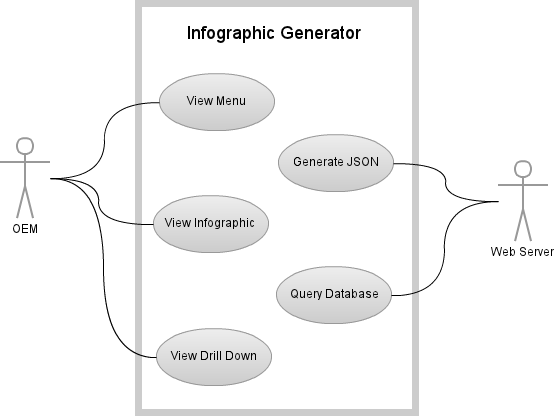
\includegraphics[width=1\textwidth]{images/Capstone_-_Use_Case_Diagram.png}\\   
\end{figure}


\subsection{System Architecture}

The infographic application is comprised of two major components: a web application/user interface and a backend database. Users are assumed to use safari browser on iPad. The web host then displays the menu screen. Data will be pulled until specific category is selected. When a category is selected, the program will pull up all the required data from the server. Depending on the style of infographic, data will be displayed in different form.\\

\subsection{User Interface}

%Figure~\ref{mockup-main-menu} 
shows the screen mockup for our prototype.  The main page will be displayed in lazy Suzan style that allows the user to scroll through the icons to the right or left.  The infographic for the current category will be shown when the icon is clicked on.\\


%Figure~\ref{mockup-infographic-display-1}, Figure~\ref{mockup-infographic-display-2}, and Figure~\ref{mockup-infographic-display-3} 
show a sample infographic depiction.  If you want to view data for another month, you can just swipe left and right to change the time frame.  If you want to go back to the main menu page, just click on the top right corner’s menu button.\\


%\begin{figure}[!]
%\caption{Main Menu Mockup\label{mockup-main-menu}}
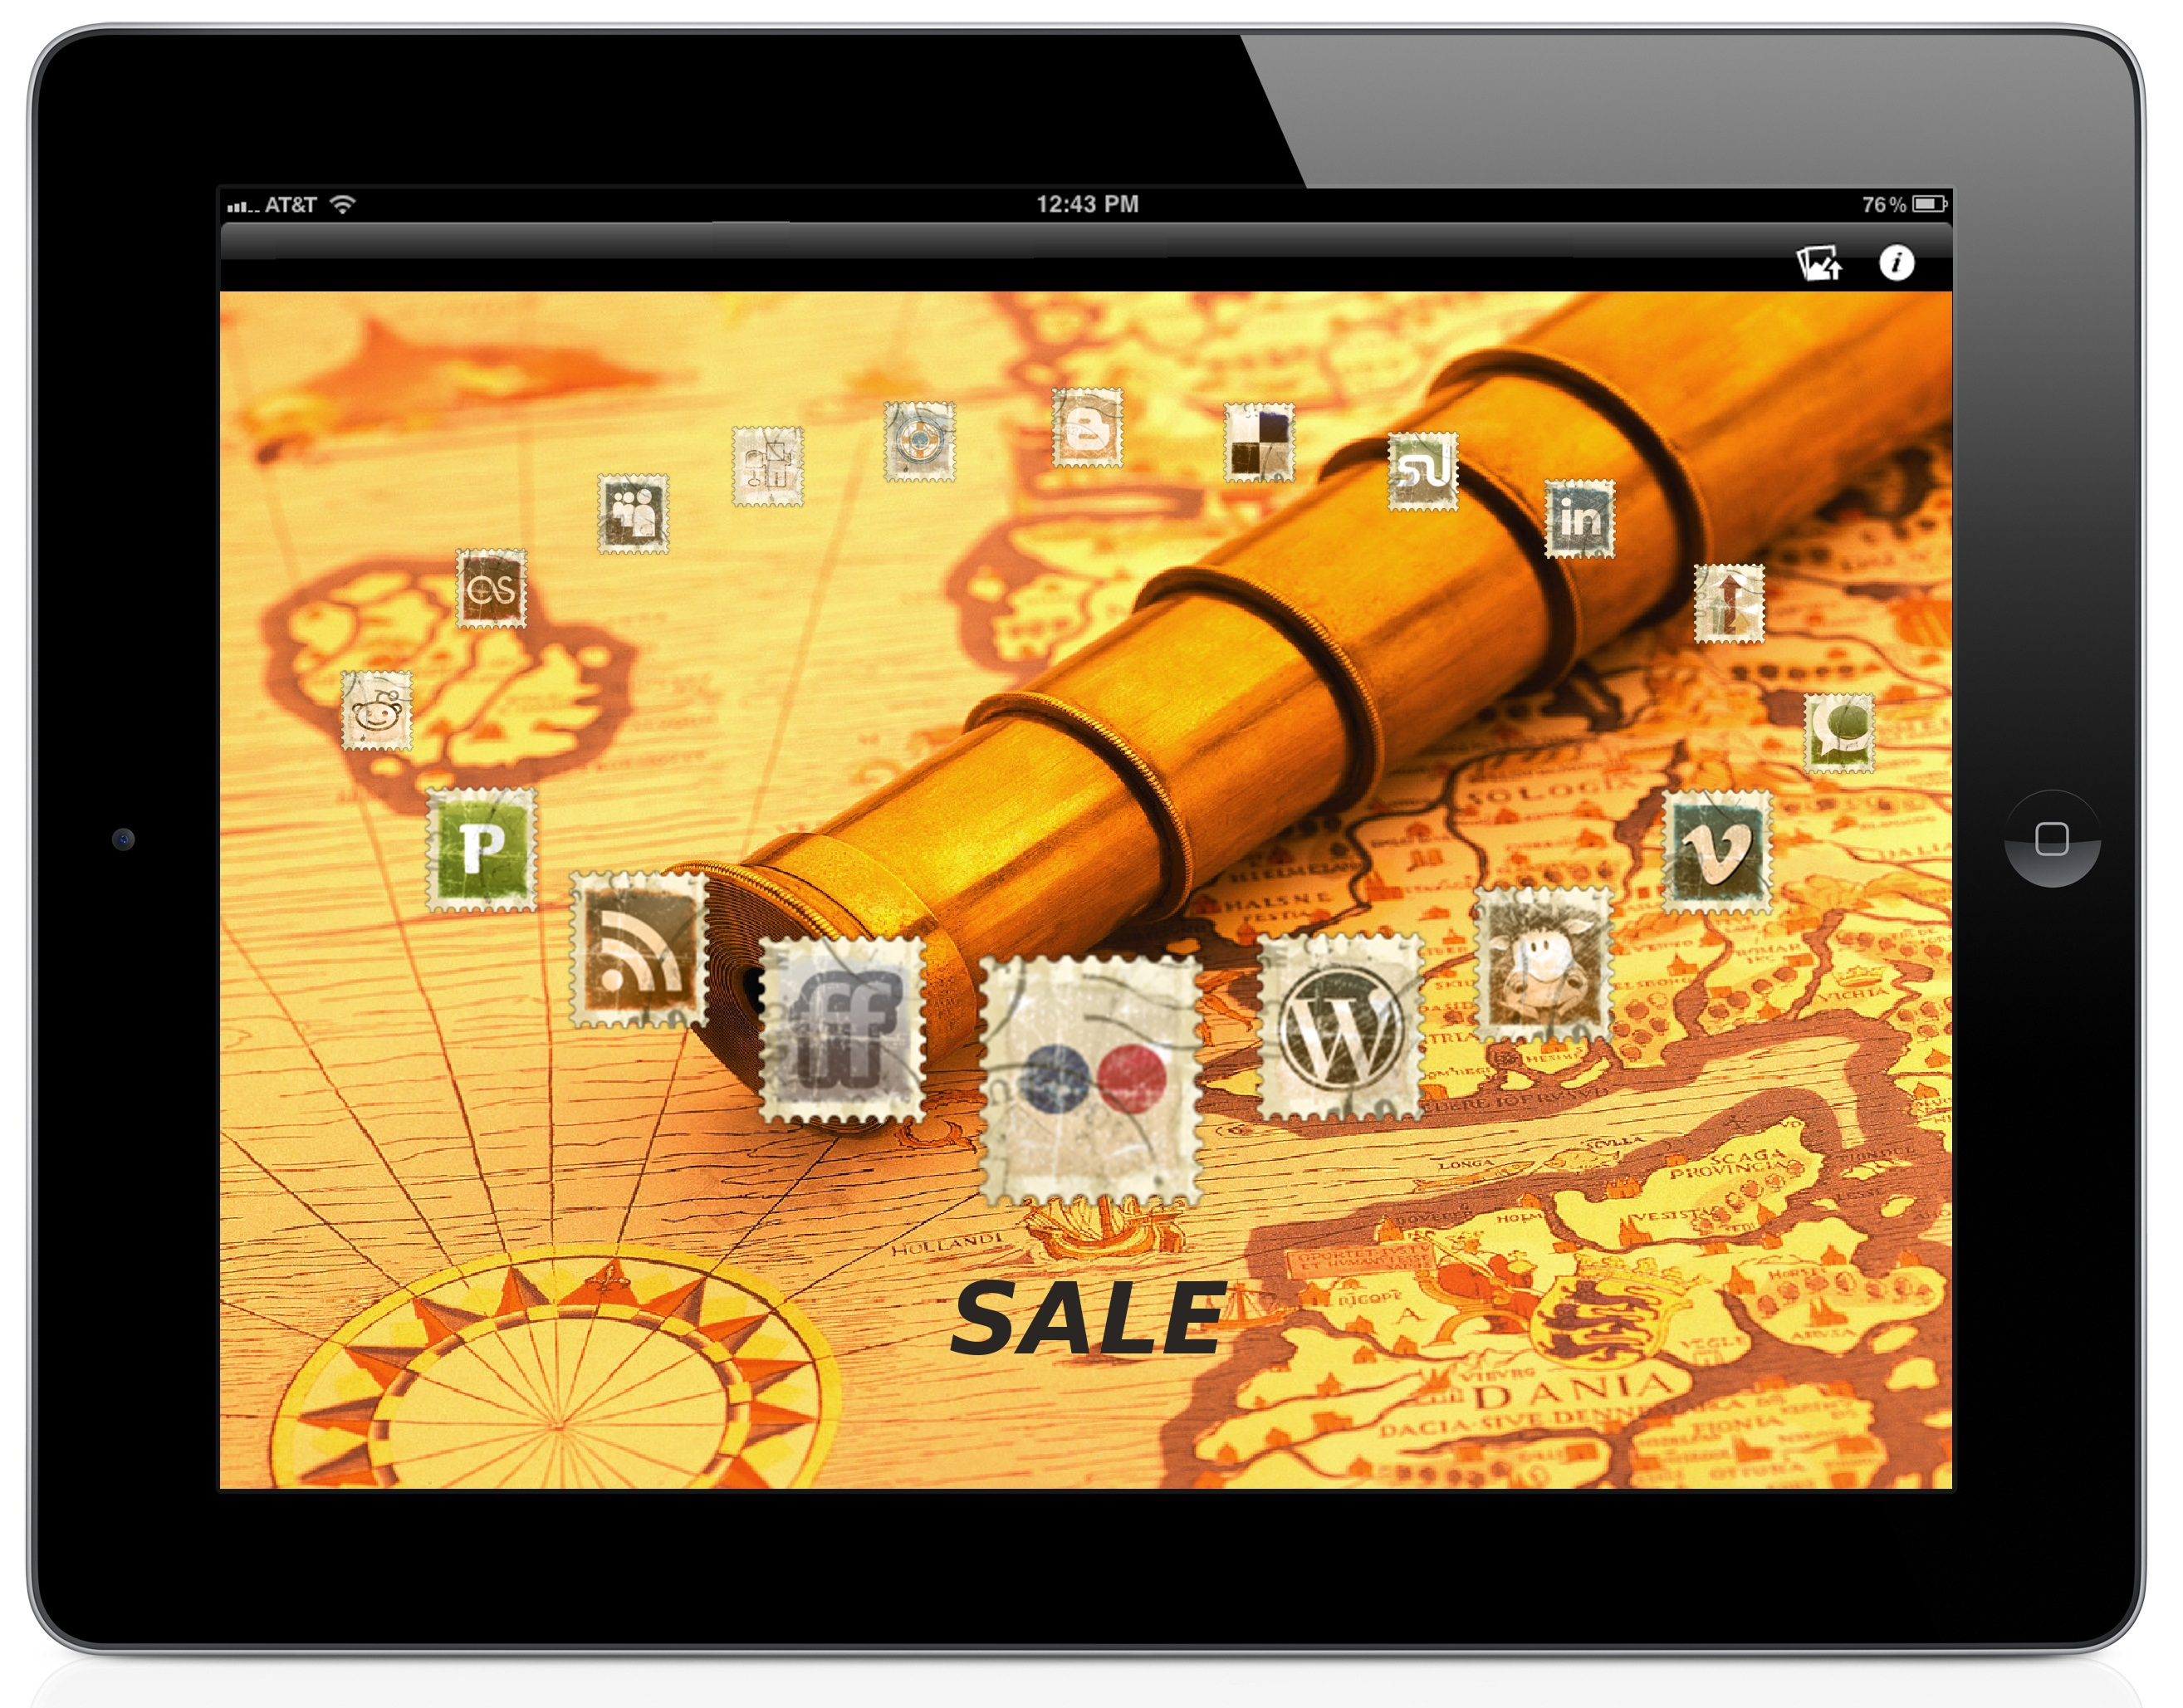
\includegraphics[width=1\textwidth]{images/screen.jpg}\\
%\end{figure}


%\begin{figure}[!]
%\caption{Infographic Display Mockup\label{mockup-infographic-display-1}}
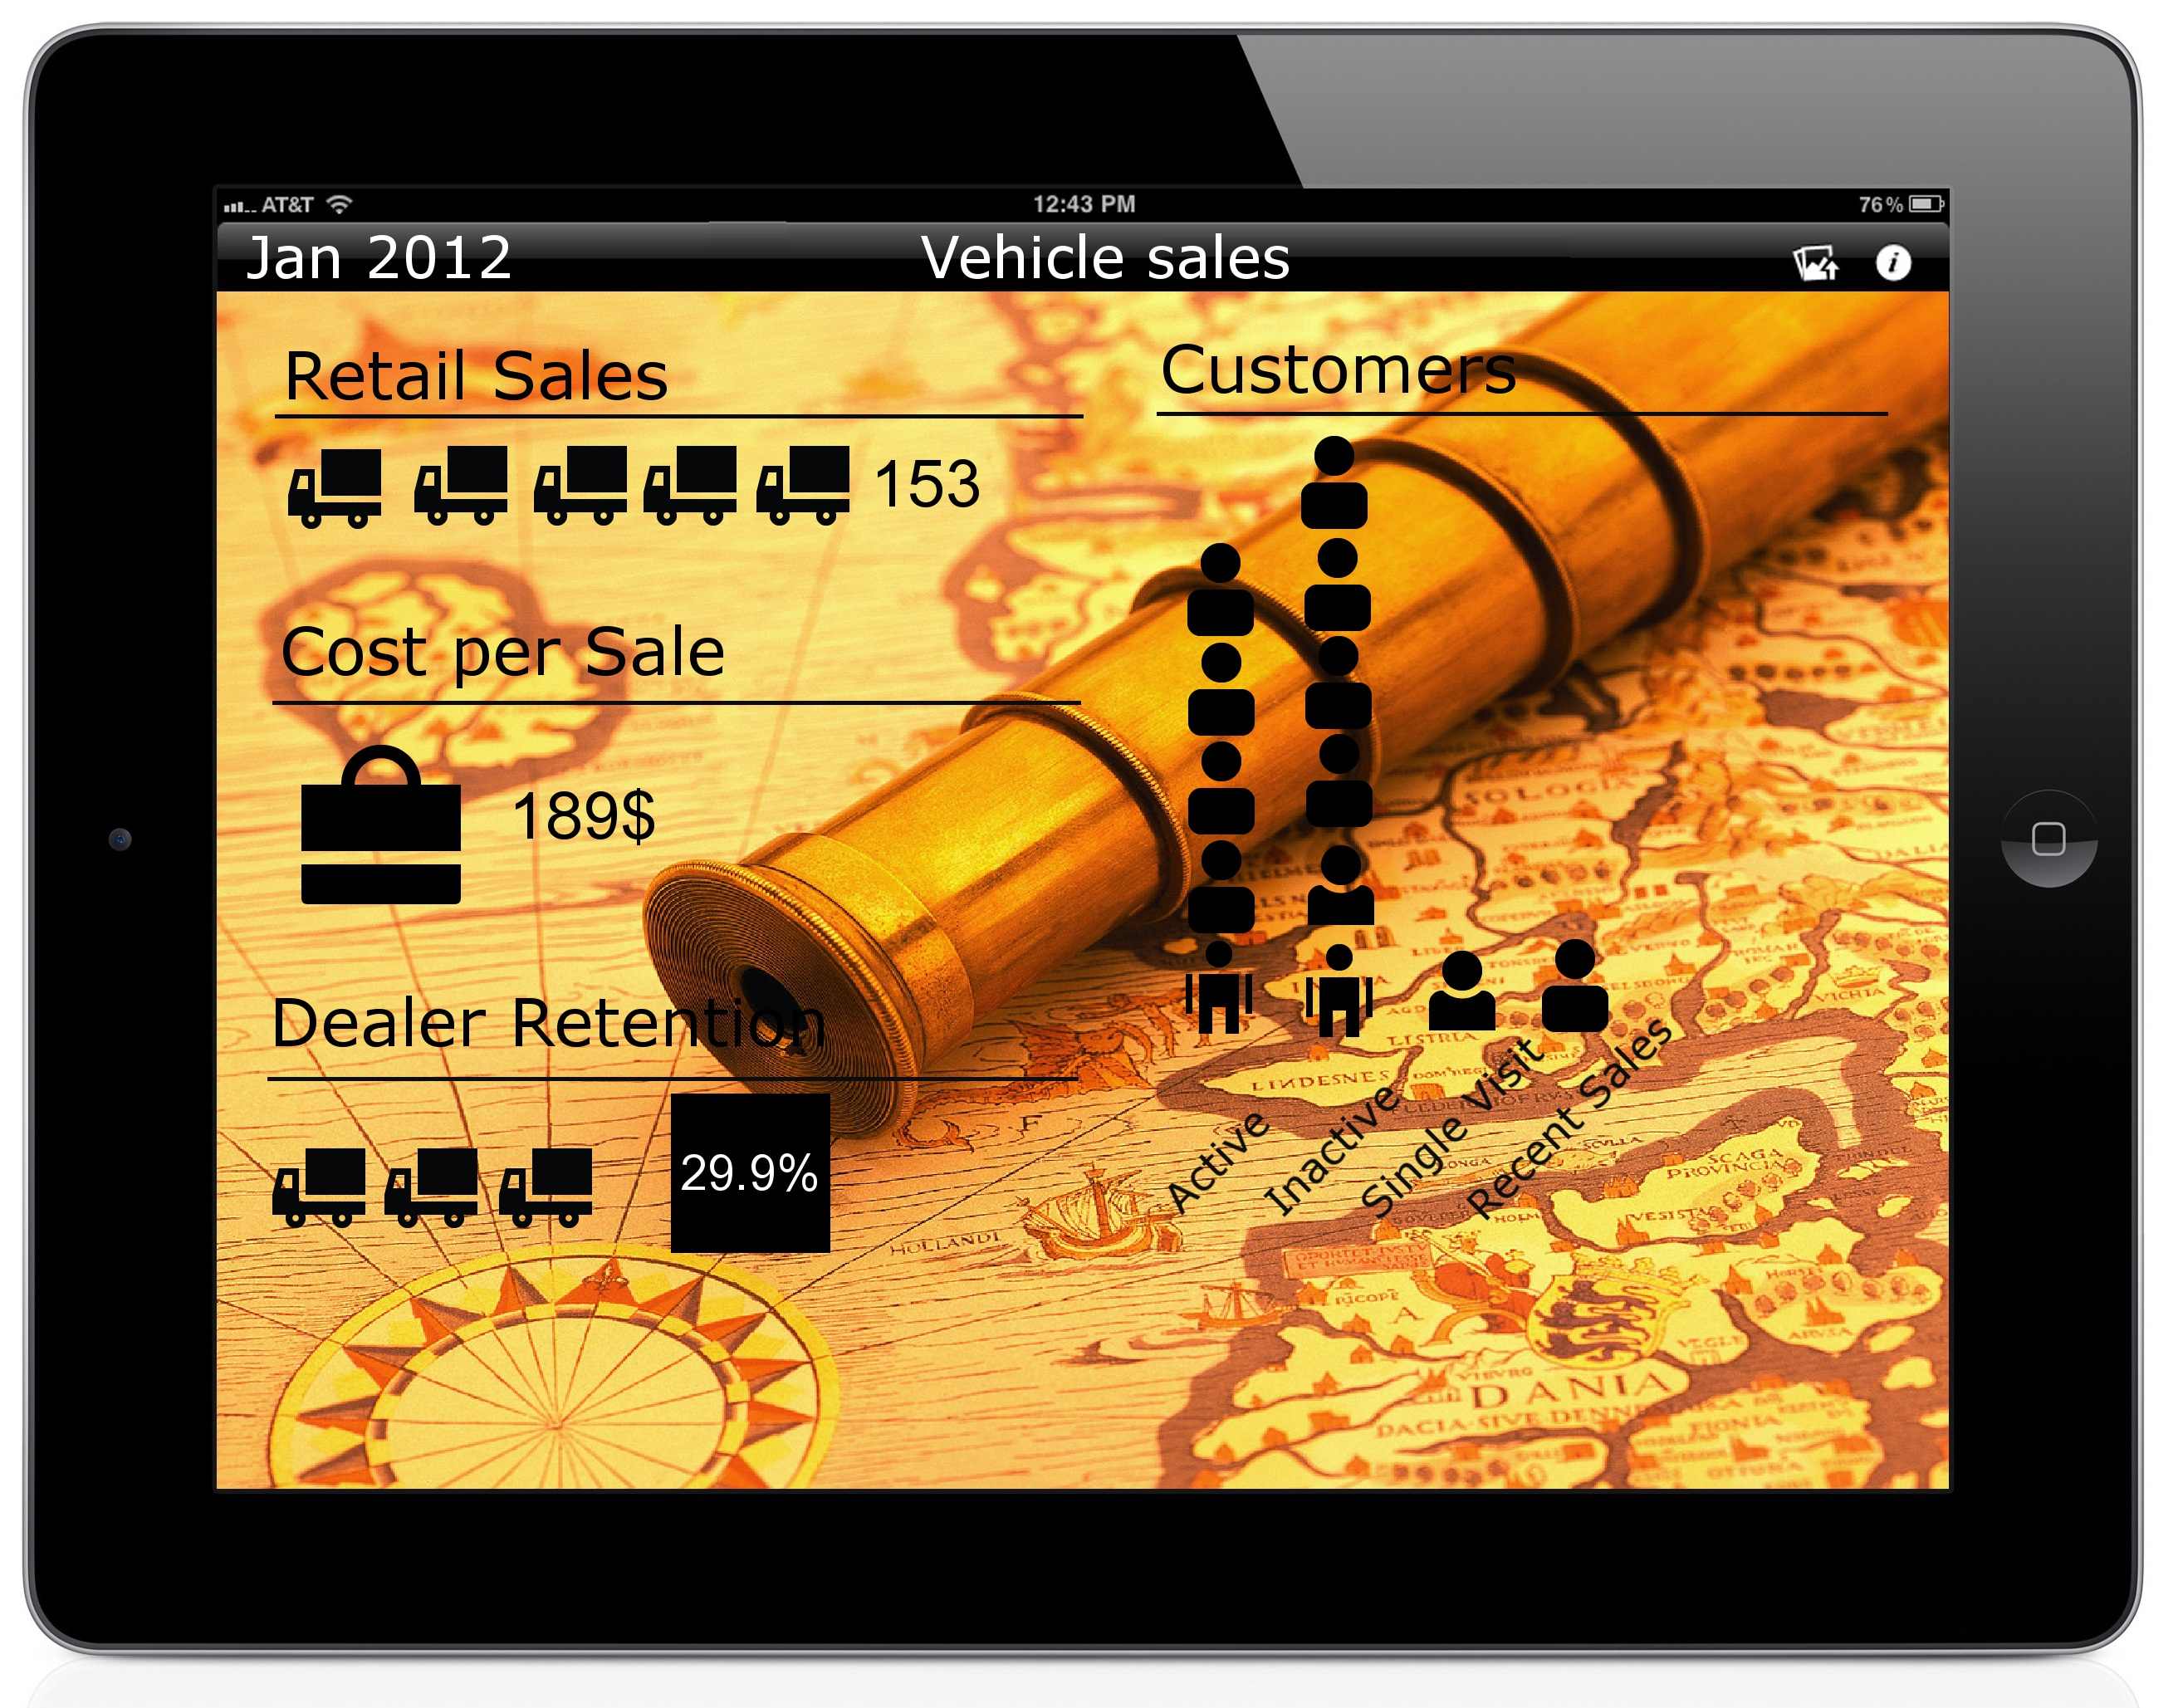
\includegraphics[width=1\textwidth]{images/screen5.jpg}\\
%\end{figure}

%\begin{figure}[!]
%\caption{Infographic Display Mockup\label{mockup-infographic-display-2}}
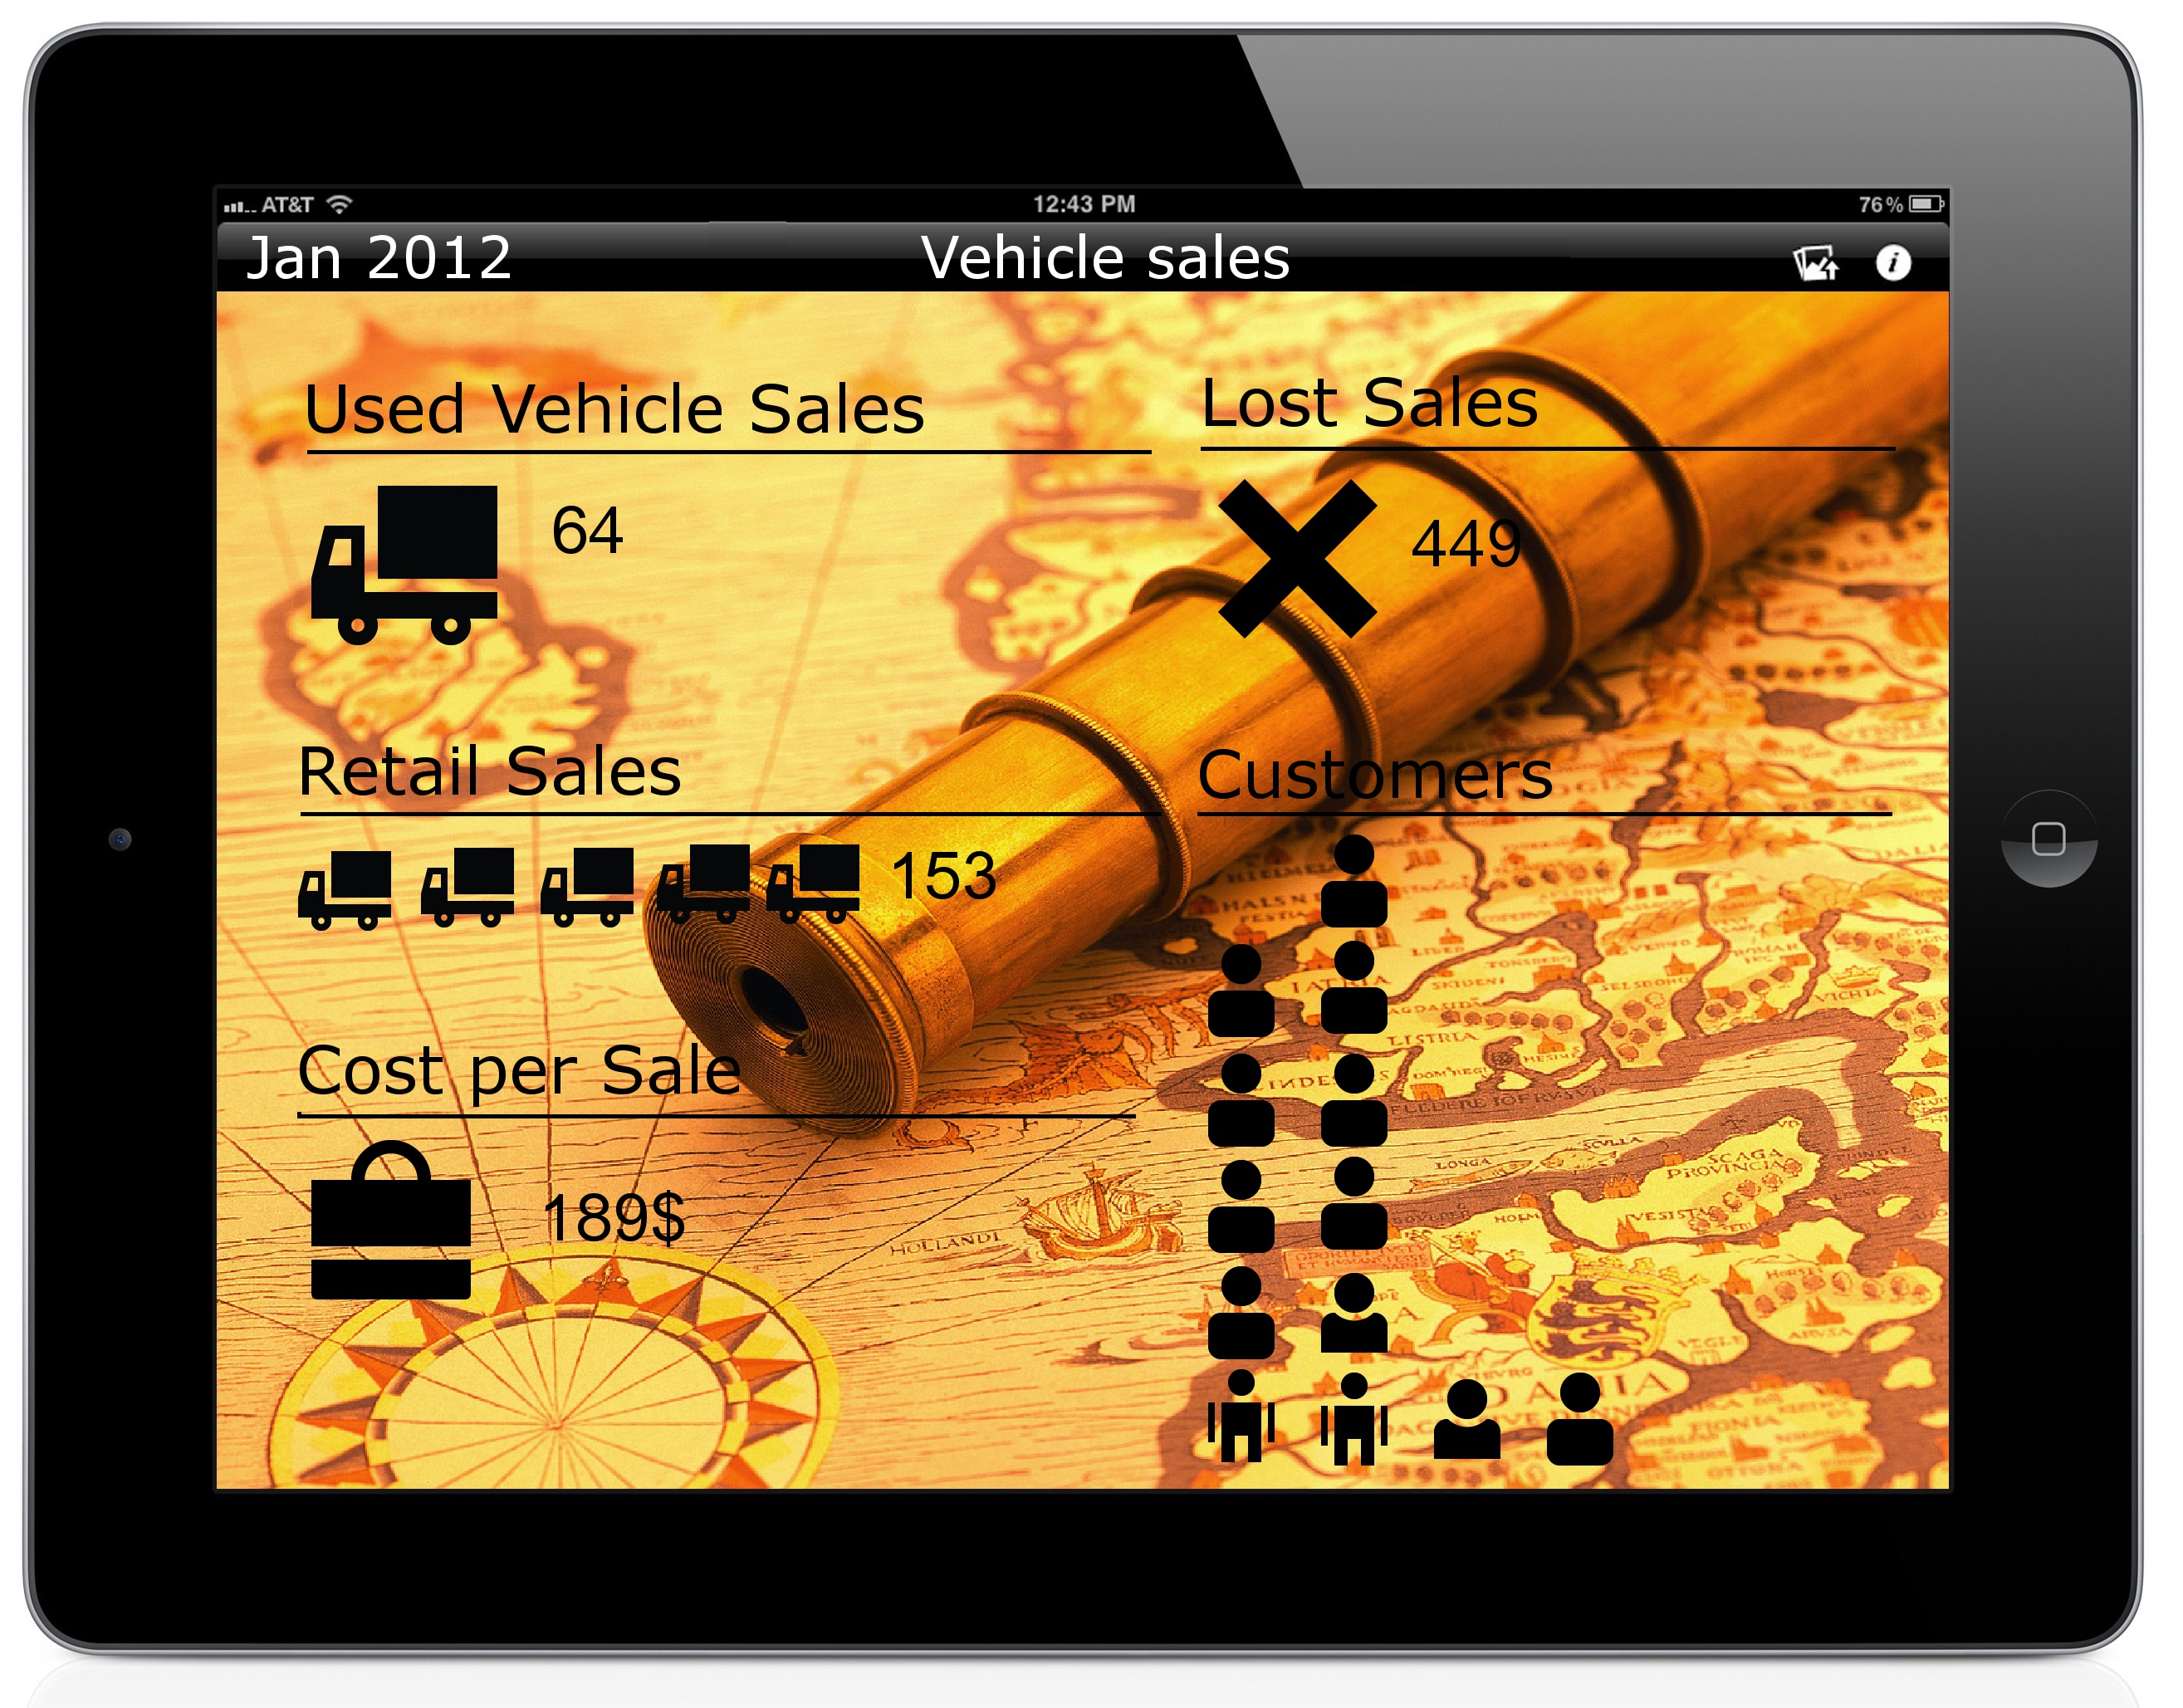
\includegraphics[width=1\textwidth]{images/screen3.jpg}\\
%\end{figure}

%\begin{figure}[!]
%\caption{Infographic Display Mockup\label{mockup-infographic-display-3}}
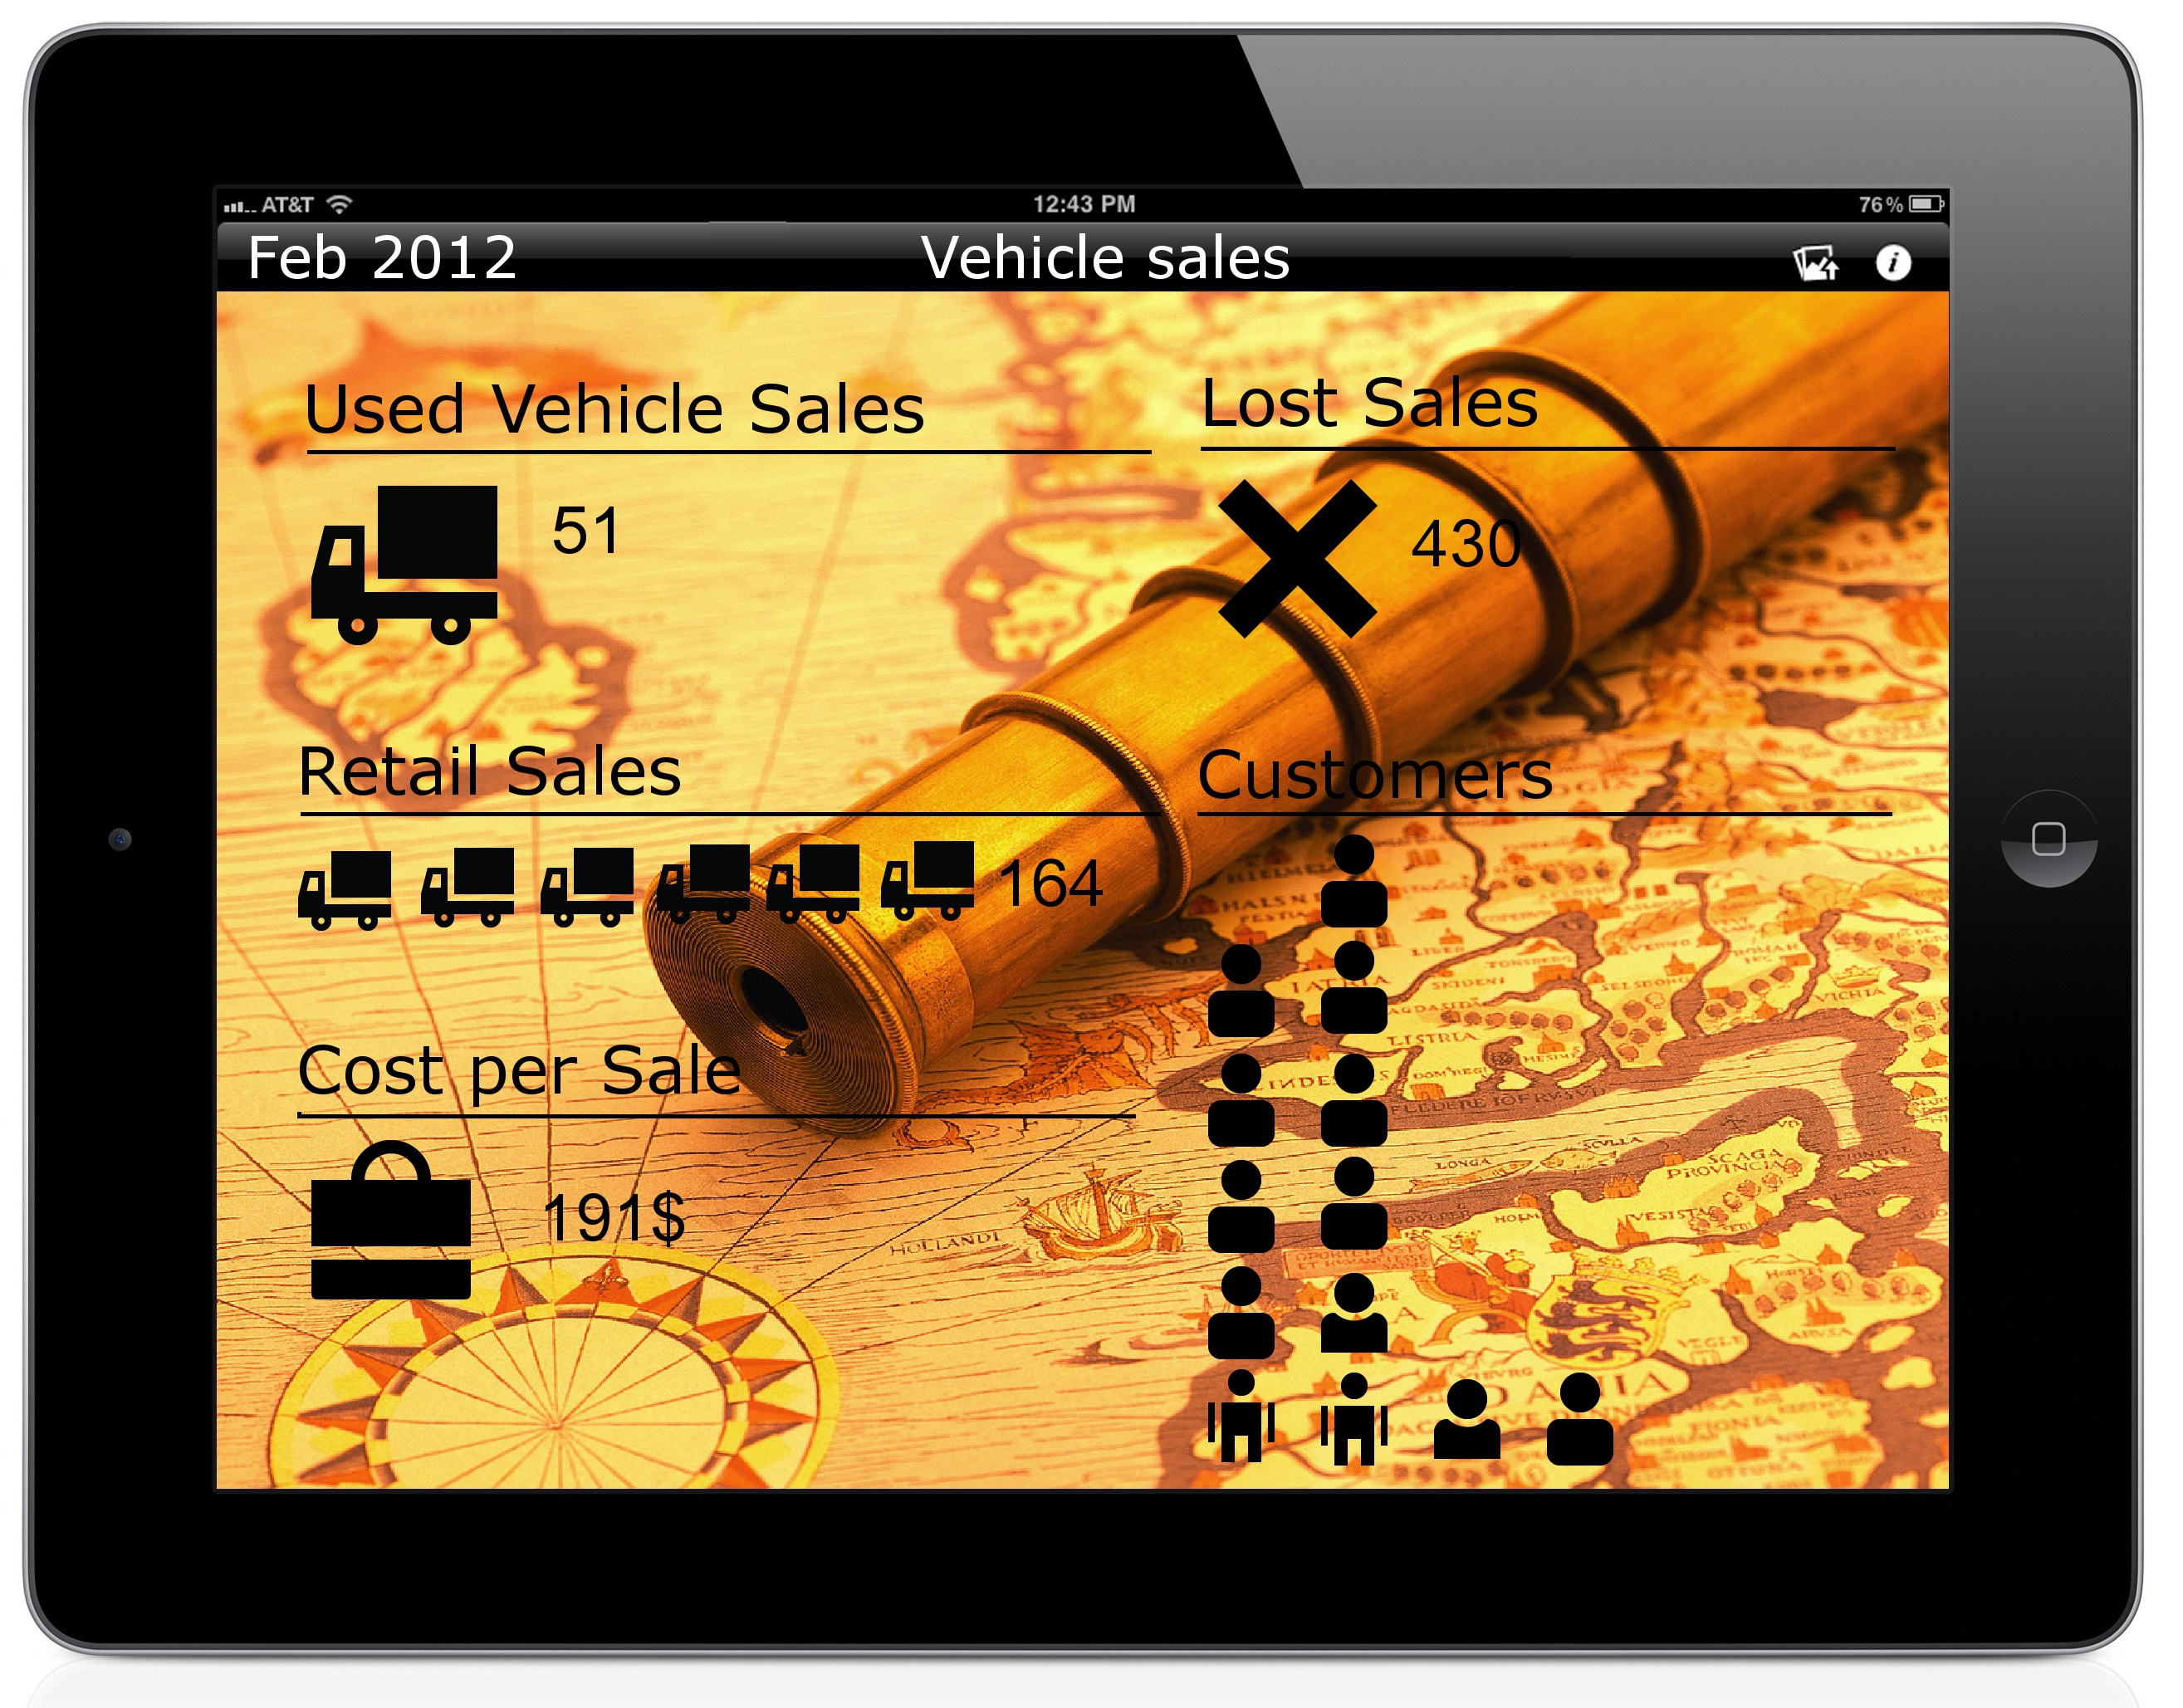
\includegraphics[width=1\textwidth]{images/screen4.jpg}\\
%\end{figure}

\section{Technical Specifications}

The infographics generator produces infographics suitable for display on the iPad 2 using the Safari browser.\\

The Index.html page in our webapp contains the infographic selector menu. The infographic selector menu is used to browse all available infographics. The infographics available to choose from include: Sales, Service, and Lead Management. The selector interface has three icons, each representing an infographic, arranged in a horizontally elongated ellipse. A swipe in the left direction causes the icons to rotate clockwise following the elliptical path. Likewise, the icons rotate counter clockwise when swiped in the right direction. This creates the illusion that the icons are rotating on an invisible lazy suzan. By swiping, the user feels that they are causing the invisible lazy suzan to rotate. Upon pressing the front most icon, Safari navigates to the corresponding infographic's page.\\


The infographic display page contains a floating image called the header. The header spans the width of the page and remains at the top of the page when the user scrolls. The header has a button on the left hand side which, if pressed, navigates back to the infographic selector menu. The right side of the header has text displaying the month and year of the data being displayed. The infographic is located immediately beneath the header and spans the entire width of the page. If the infographic is swiped left, the next month's data is displayed. If swiped right, the previous month's data is displayed. If no data exists for the month attempting to be displayed, the current date is not changed.\\


Each infographic displays multiple key performance indicators (KPI) data. The data is obtained from a Microsoft SQL database. The server hosting the infographics generator uses an ASP.NET script (KPI\_Handler.ashx) to query the database for all available KPI data, serializes the data, and returns the data to the client device in JavaScript Object Notation (JSON). The client device then parses this data using a JavaScript function (found in Scripts/KPILocalStorage.js) and adds the data to local storage.\\


An infographic element is a visual representation of KPI data, responsible for displaying one or more KPI data. An infographic is comprised of multiple infographic elements. Each infographic element is drawn on an HTML5 canvas using JavaScript functions found in one of the three infographic drawing files (draw-sales.js, draw-service.js, draw-lead.js) or the common element file (elements.js). The common element file is used to centralize the generic JavaScript functions that are used to draw the elements in the infographics. The infographic specific files call functions from the common element file and have their own JavaScript functions to draw the infographic. They also calls functions to retrieve specific KPI values from local storage.\\


A drill down display is shown in the center of the screen if an infographic element is tapped. The drill down display gives an brief description of the KPI that was tapped and shows a trend chart of the KPI over the last 6 months (ending in the current month) or the maximum number of months available, whichever number is smaller.\\




\begin{figure}[!]
\caption{Sequence Diagram}
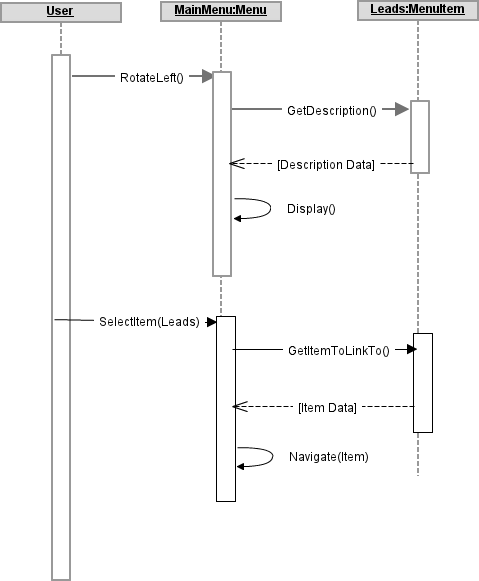
\includegraphics[width=1\textwidth]{images/Capstone_-_Sequence_Diagram.png}\\
\end{figure}


\begin{figure}[!]
\caption{Class Diagram}
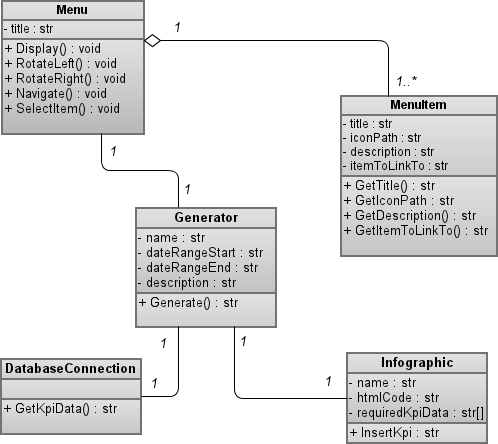
\includegraphics[width=1\textwidth]{images/Capstone_-_Class_Diagram.png}\\
\end{figure}


\section{Schedule}

\subsection{Week 1 (January 9, 2012)}
\begin{itemize}
\item Had our first conference call with our customer
\item Set up weekly conference calls with our customer
\item Set up regular team meetings to meet twice a week
\item Installed virtual machines
\end{itemize}


\subsection{Week 2 (January 16, 2012)}
\begin{itemize}
\item Started UML diagrams
\item Installed Windows Server 2008 R2
\item Installed IIS 7
\item Installed ASP.NET
\item Installed Microsoft SQL Server
\item Talked with our customer about interface mockups
\end{itemize}

\subsection{Week 3 (January 23, 2012)}
\begin{itemize}
\item Completed more UML diagrams
\item First draft of project-plan
\item Installed Visual Studio 2010
\item Created screen mockups
\item Created sample infographic elements
\end{itemize}

\subsection{Milestone: Status Reports}
\begin{itemize}
\item Gave report to class
\end{itemize}

\subsection{Week 4 (January 30, 2012)}
\begin{itemize}
\item Created infographic elements using actual KPI data
\item Wrote website to showcase infographics
\item Decided to work on sales infographic first
\end{itemize}

\subsection{Milestone: Project Plan Presentation}
\begin{itemize}
\item Gave presentation in class
\end{itemize}

\subsection{Week 5 (February 6, 2012)}
\begin{itemize}
\item Presented project plan to class
\item Changed from using XML to JSON for pulling database information
\item Have roundabout working with several images for infographic selector buttons
\item Successfully pulled data from a SQL database using ASP.NET
\end{itemize}

\subsection{Week 6 (February 13, 2012)}
\begin{itemize}
\item Sales infographic exists in basic form
\item Added background image to main menu
\end{itemize}

\subsection{Week 7 (February 20, 2012)}
\begin{itemize}
\item Infographics now use values from database
\item Rewrote pump in sales infographic
\item Practiced Alpha Demonstration
\end{itemize}

\subsection{Milestone: Alpha Demonstrations}
\begin{itemize}
\item Demonstrated software to Urban Science for first time
\item Recieved usefull feedback from Urban Science
\end{itemize}

\subsection{Week 8 (February 27, 2012)}
\begin{itemize}
\item Planning for betas
\item Created mockups of service and lead management infographics
\end{itemize}

\subsection{Week 9 (March 12, 2012)}
\begin{itemize}
\item Added service infographic to website
\item Fixed bugs with swiping
\item Local storage now refreshes with website
\end{itemize}

\subsection{Week 10 (March 19, 2012)}
\begin{itemize}
\item Added MSU and Urban Science branding to website
\item Visited Urban Science headquarters in Detroit, MI
\end{itemize}

\subsection{Week 11 (March 26, 2012)}
\begin{itemize}
\item Added remaining KPI to service and lead management infographics
\item Implemented drill down display
\item Began writing script for video
\item Practiced for Beta presentation
\end{itemize}

\subsection{Milestone: Beta Demonstrations}
\begin{itemize}
\item Presentation was successful
\item Project was feature complete
\end{itemize}

\subsection{Week 12 (April 2, 2012)}
\begin{itemize}
\item Changed text formatting upon customer request
\item Fixed bugs with swiping 
\end{itemize}

\subsection{Week 13 (April 9, 2012)}
\begin{itemize}
\item Updated project plan to reflect most recent version of webapp
\item Discovered origin of grey background in jQuery css file
\end{itemize}

\subsection{Week 14 (April 16, 2012)}
\begin{itemize}
\item Has not occured
\end{itemize}

\subsection{Week 15 (April 23, 2012)}
\begin{itemize}
\item TODO: clean up code
\item TODO: write documentation for functions
\item TODO: project video
\item TODO: rename /webapp/images/avg\$.png because of potential problems with having a dollar sign in the filename
\end{itemize}

\subsection{Milestone: Projet Video}
\begin{itemize}
\item Has not occured
\end{itemize}

\subsection{Milestone: All Deliverables}
\begin{itemize}
\item Has not occured
\end{itemize}

\subsection{Milestone: Design Day}
\begin{itemize}
\item Has not occured
\end{itemize}




\section{Remaining tasks}
\begin{itemize}
\item clean up code
\item write documentation for functions
\item project video
\item rename /webapp/images/Avg\$.png because of potential problems with having a dollar sign in the filename
\item make close rate a percentage
\end{itemize}


\end{document}
